% !TEX program = pdflatex
% AAAI-27 anonymous submission source (main paper, 7 pages of body, 9 pages total).
% Compile with pdfLaTeX + BibTeX (aaai2027.bst). Requires aaai2027.sty and
% aaai2027.bst in the same directory (from the official AAAI Author Kit 2027).
\documentclass[letterpaper]{article} % DO NOT CHANGE THIS
\usepackage[submission]{aaai2027}  % DO NOT CHANGE THIS
\usepackage[hyphens]{url}  % DO NOT CHANGE THIS
\usepackage{graphicx} % DO NOT CHANGE THIS
\urlstyle{rm} % DO NOT CHANGE THIS
\def\UrlFont{\rm}  % DO NOT CHANGE THIS
\usepackage{natbib}  % DO NOT CHANGE THIS
\usepackage{caption} % DO NOT CHANGE THIS
\frenchspacing  % DO NOT CHANGE THIS
\usepackage{booktabs}
\usepackage{array}
\usepackage{amsmath,amssymb}
\usepackage{enumitem}

\pdfinfo{
/TemplateVersion (2027.1)
}

\setcounter{secnumdepth}{1}

\title{Bidirectional Sub-Answer Cross-Checking for Multi-Hop QA on Long Multi-Document Contexts}
\author{
    Anonymous Submission
}
\affiliations{
}

\begin{document}
\maketitle

\begin{abstract}
Multi-hop question answering on long multi-document contexts (5--12k tokens, e.g., retrieval-augmented QA over multi-domain passages) poses a challenge that neither Chain-of-Thought (CoT) nor Self-Consistency (CoT-SC) resolves: relevant evidence is scattered across passages with heavy distractors, and quality-agnostic majority voting cannot separate a grounded reasoning path from a confidently wrong one. We propose \textbf{GERS-CV2}, which decomposes the question into a dependency DAG, executes sub-questions in topological order, and verifies each sub-answer via \textbf{bidirectional cross-checking}: using the final answer and context as an anchor, each sub-question is re-derived in reverse, and forward/backward agreement forms a content self-consistency score. On LongBench, GERS-CV2 significantly outperforms CoT-SC on two independent English multi-document QA subsets under paired evaluation: multifieldqa\_en (n=100, F1 +0.070, 95\% CI $[+0.007, +0.132]$) and musique (n=193, F1 +0.063, 95\% CI $[+0.001, +0.124]$, McNemar $p=0.049$). To explain \emph{why} decomposition helps, an Oracle analysis on MuSiQue 4-hop (n=200) shows that substituting gold decomposition into our pipeline yields a paired-significant +0.075 F1 gain over CoT-SC (95\% CI $[+0.017, +0.134]$), directly demonstrating that decomposition itself is valuable when done well; a per-module waterfall further localizes 66\% of recoverable F1 to reasoner error propagation---exactly the failure mode that bidirectional cross-checking targets. The cross-check also raises the Consistency Score's correct/wrong discrimination from $-0.0035$ (structural baseline) to $+0.0847$ (AUROC 0.498$\to$0.589). We honestly delineate the method's regime: it does not improve on short evidence-dense contexts (HotpotQA), reaches a joint model-capacity ceiling on ultra-long single-narrative texts, and compresses toward zero on stronger base models.
\end{abstract}

\section{Introduction}

Multi-hop question answering requires combining evidence from multiple passages, and is central to evaluating LLM reasoning. Chain-of-Thought (CoT) prompting~\citep{wei2022cot} elicits intermediate steps; Self-Consistency (CoT-SC)~\citep{wang2023sc} samples multiple paths and takes the majority answer. Both are strong baselines when evidence is concentrated in a short, dense passage. But in the operationally important regime of \textbf{long multi-document contexts}---the setting produced by retrieval-augmented generation over multi-domain corpora, captured by benchmarks such as LongBench~\citep{bai2024longbench}---these baselines face two compounding challenges:

\begin{enumerate}[leftmargin=*,topsep=0pt,itemsep=1pt]
\item \textbf{Attention dilution across passages.} When relevant evidence is scattered across 5--12k tokens of multi-domain context with heavy distractors, single-pass reading dilutes attention and single-shot CoT frequently misses cross-passage bridging entities.
\item \textbf{Vote noise on confidently wrong paths.} CoT-SC's equal-weighted majority vote cannot distinguish a grounded reasoning path from a fluent hallucination; three confidently wrong samples can outvote one correct sample.
\end{enumerate}

Graph-based reasoning has been proposed as an alternative: GoT~\citep{besta2024got} allows merging and distillation of thoughts; RwG~\citep{han2025rwg} structures the context into an entity-relation graph; MoDeGraph~\citep{oruche2025modegraph} builds a multi-hop dependency graph as a prompt. These approaches share the intuition that structuring reasoning should help, but leave open whether graph decomposition, executed with topological ordering, actually beats CoT-SC under \emph{fair paired evaluation on the target regime}, and whether the graph can produce a useful \emph{content-level} consistency signal despite the fact that purely structural graph-validity metrics are known to be non-discriminative (LLM-generated graphs are almost always legal DAGs).

We answer both questions affirmatively. We propose \textbf{GERS-CV2}, whose central mechanism is \textbf{bidirectional sub-answer cross-checking}: after the forward pass produces a final answer $A$, each sub-question is re-derived \emph{in reverse}, using $A$ and the context as an anchor; the agreement between forward and backward sub-answers is aggregated into a content self-consistency score. This cross-check is directly enabled by explicit DAG decomposition---the DAG exposes named, individually checkable sub-question units---and does not apply naturally to unstructured linear CoT.

\noindent\textbf{Contributions.}
\begin{enumerate}[leftmargin=*,topsep=0pt,itemsep=1pt]
\item \emph{A method that significantly wins on long multi-document QA.} On the LongBench multi-document QA regime under fair full-context paired evaluation, GERS-CV2 significantly outperforms CoT-SC on two independent subsets: multifieldqa\_en (n=100, F1 +0.070, 95\% CI $[+0.007, +0.132]$) and musique (n=193, F1 +0.063, 95\% CI $[+0.001, +0.124]$, McNemar $p=0.049$).
\item \emph{A mechanism explanation via Oracle analysis.} Substituting gold decomposition on MuSiQue 4-hop (n=200) into our pipeline yields a paired-significant +0.075 F1 gain over CoT-SC, directly quantifying decomposition's method value. A per-module waterfall identifies the reasoner (66\%) as the dominant recoverable factor---the exact module bidirectional cross-checking targets.
\item \emph{A repaired consistency signal.} Bidirectional cross-checking raises the Consistency Score's correct/wrong discrimination from $-0.0035$ (structural baseline) to $+0.0847$, and AUROC from 0.498 to 0.589, upgrading it from an uninformative graph-validity metric to a diagnostic content self-consistency signal.
\item \emph{Honest regime boundaries.} We explicitly delineate where the method does not help: HotpotQA (short single-file dense evidence), narrativeqa ($>$22k tokens, exceeds 8B-model usable attention), and stronger models where CoT-SC already saturates.
\end{enumerate}

\section{Related Work}

\noindent\textbf{Chain-of-Thought reasoning.} \citet{wei2022cot} introduced CoT prompting; \citet{wang2023sc} proposed Self-Consistency (CoT-SC), whose equal-weight majority vote does not exploit path quality. \citet{yao2023tot} proposed Tree of Thoughts (ToT) with search over thought states, without explicit sub-question dependency modeling. These methods are based on linear or tree structures.

\noindent\textbf{Graph-enhanced reasoning.} \citet{besta2024got} models reasoning as a graph for merging/distillation, focused on prompt engineering. \citet{han2025rwg} uses a context graph as a one-time input. \citet{oruche2025modegraph} builds a multi-hop dependency graph as a prompt method. Unlike these, GERS couples the reasoning graph with sub-question execution \emph{and} designs a content-level consistency signal (bidirectional cross-checking) that exploits the DAG's individually-checkable sub-question structure.

\noindent\textbf{Long-context QA benchmarks.} LongBench~\citep{bai2024longbench} is a bilingual multi-task long-context benchmark; MuSiQue~\citep{trivedi2022musique} composes single-hop questions into 2--4-hop compositions with gold sub-question decompositions. We use LongBench multi-document QA subsets as the main benchmark, and MuSiQue for controlled Oracle mechanism analysis.

\noindent\textbf{Consistency checking and self-evaluation.} Process Reward Models~\citep{lightman2024verify} score intermediate steps but require large amounts of labeled data. Self-Refine~\citep{madaan2023selfrefine} iteratively refines answers via self-feedback on linear text. GERS designs bidirectional sub-answer cross-checking, made possible by explicit DAG decomposition.

\section{Method}

\subsection{Overall Framework}

Given question $Q$ and context $C$, GERS-CV2 executes: (1) decompose $Q$ into ordered sub-questions $\{q_i\}$ with dependencies; (2) build DAG $G=(V,E)$; (3) topological sort $\tau$; (4) execute sub-questions in order, injecting predecessor answers as context, producing sub-answers $\{a_i\}$; (5) aggregate into final answer $A$ (with answer-type alignment to the original question); (6) compute the cross-validated Consistency Score $S = 0.3\cdot S_{\text{struct}} + 0.7\cdot S_{\text{crossval}}$. Figure~\ref{fig:framework} depicts the pipeline.

\begin{figure}[t]
\centering
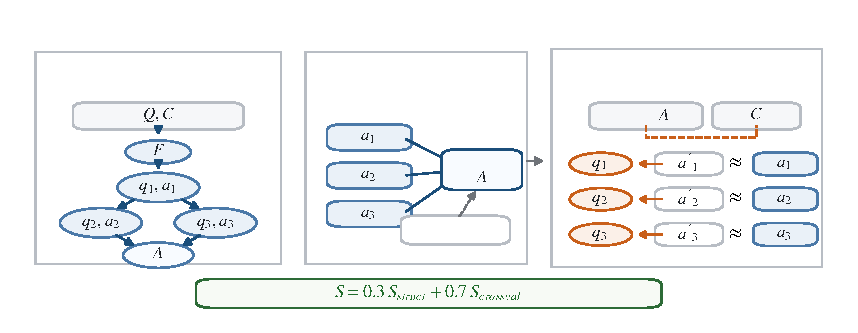
\includegraphics[width=0.98\linewidth]{figures/image1}
\caption{GERS-CV2 pipeline. A question is decomposed into a dependency DAG, executed in topological order, aggregated into a final answer, then verified by bidirectional cross-checking anchored on the final answer and context.}
\label{fig:framework}
\end{figure}

\subsection{Reasoning-State Graph}

Nodes: \emph{FactNode} (facts/original question), \emph{StepNode} (sub-question and answer), \emph{ConclusionNode} (final conclusion). Edges: \emph{DeriveEdge}, \emph{SupportEdge}, \emph{ConflictEdge}. The LLM decomposes $Q$ into an ordered sub-question list with dependencies; nodes and edges are created accordingly. Topological sort orders execution; cycles are broken first.

\subsection{Bidirectional Sub-Answer Cross-Checking}

\noindent\textbf{Structural score (baseline).}
$S_{\text{struct}} = w_1 C_{\text{conn}} + w_2 C_{\text{cycle}} + w_3 C_{\text{cov}}$
with $w_1{=}w_3{=}0.35, w_2{=}0.30$ for connectivity, acyclicity, and coverage. On our data this metric clusters (mean 0.66, discrimination $-0.0035$) and cannot distinguish reasoning quality.

\noindent\textbf{Bidirectional cross-check (core).} Given forward sub-answers $\{a_i\}$ and final answer $A$, each sub-question is re-answered \emph{in reverse} using ``$A$ + context $C$'' as anchor, yielding backward sub-answers $\{a'_i\}$. Content consistency is
\begin{equation}
S_{\text{crossval}} = \frac{\sum_{i=1}^{n} w_i \cdot \mathbb{1}[\text{match}(a_i, a'_i)]}{\sum_{i=1}^{n} w_i}
\end{equation}
with $w_i = 0.5 + 0.5\cdot(i+1)/n$ (downstream sub-questions weighted higher, since their errors propagate further). The match function is a three-level heuristic: (i) exact match after normalization (lowercasing, punctuation removal, yes/no and numeric unification), (ii) substring containment or numeric equality, (iii) otherwise 0. The reverse prompt explicitly instructs ``re-derive from context, do not copy $A$'' to mitigate confirmation bias.

\begin{figure}[t]
\centering
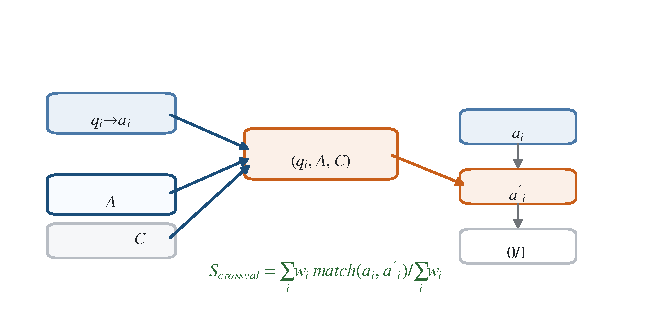
\includegraphics[width=0.98\linewidth]{figures/image3}
\caption{Bidirectional sub-answer cross-checking. Forward pass produces sub-answers and final answer $A$; each sub-question is re-derived in reverse anchored on ``$A$ + context''. Agreement between forward and backward yields a content self-consistency score.}
\label{fig:crosscheck}
\end{figure}

\noindent\textbf{Confidence-weighted aggregation.} Each sub-answer is scored by a lightweight heuristic (non-emptiness, absence of uncertainty markers, entity grounding in context, pure-number check); sub-answers below $\theta_{\text{conf}}{=}0.5$ are tagged \texttt{[LOW CONFIDENCE]} in the aggregation prompt.

\section{Experiments}

\subsection{Setup}

\noindent\textbf{Main benchmarks (LongBench English QA).} We evaluate on LongBench~\citep{bai2024longbench}: \emph{multifieldqa\_en} (n=100, median $\sim$5k tok, multi-domain distractor passages) and \emph{musique} (n=200, median $\sim$11k tok, deep-hop over multiple Wikipedia passages), the two subsets in the target regime; and \emph{narrativeqa} (n=100, median $\sim$22k tok, single-narrative books) as a model-capacity ceiling.

\noindent\textbf{Mechanism benchmark.} MuSiQue~\citep{trivedi2022musique} 4-hop subset (first 200 samples with hop=4 from a seed=42 shuffle of the \texttt{musique\_ans\_v1.0\_dev} split) for the controlled Oracle study, since gold sub-question decompositions and supporting-fact annotations are available.

\noindent\textbf{Regime-boundary benchmark.} HotpotQA~\citep{yang2018hotpotqa} n=500 (single-file dense evidence, mean $\sim$4.7k characters) as a documented boundary where decomposition does not help.

\noindent\textbf{Baselines.} CoT-SC ($N{=}3$, majority vote) is the primary paired-comparison baseline. Standard CoT and Zero-Shot appear in ablations.

\noindent\textbf{Model and protocol.} Qwen3-8B via DashScope API, 4-worker parallel execution. For LongBench, both CoT-SC and GERS-CV2 see the \emph{full} context via the LongBench \texttt{context\_full} field, ensuring paired fairness (no unequal truncation confound). Answer extraction and normalization use one unified pipeline across all methods. All main comparisons report paired bootstrap 95\% CIs (B=10{,}000 resamples of per-sample differences, seed=42) and paired McNemar tests on EM correctness (chi-square with Edwards' continuity correction).

\subsection{Main Results}

\begin{figure}[t]
\centering
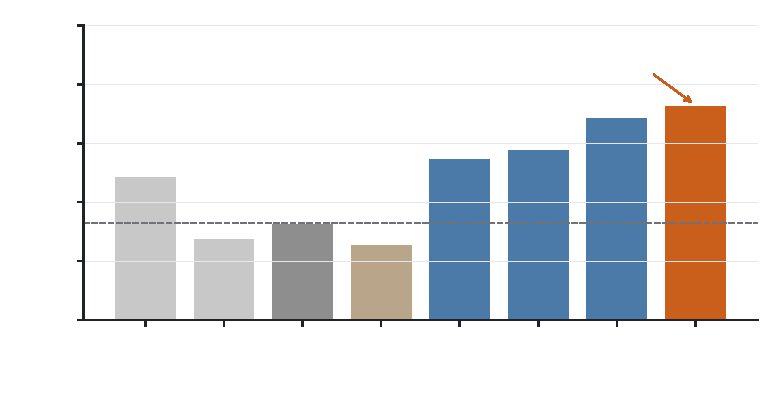
\includegraphics[width=0.98\linewidth]{figures/image4}
\caption{Main results on LongBench English multi-document QA (fair full-context evaluation, Qwen3-8B). GERS-CV2 significantly beats CoT-SC on the two target-regime subsets; narrativeqa is a joint model-capacity ceiling reported honestly.}
\label{fig:main}
\end{figure}

\begin{table*}[t]
\centering
\caption{Main results on LongBench English multi-document QA. All comparisons are paired. Bootstrap 95\% CIs exclude zero for both target-regime rows.}
\label{tab:main}
\small
\begin{tabular}{lcccccccc}
\toprule
Subset & Median tok & $n$ & CoT-SC EM/F1 & \textbf{GERS-CV2 EM/F1} & $\Delta$F1 & F1 95\% CI & McN $p$ & Verdict \\
\midrule
multifieldqa\_en & $\sim$5000 & 100 & 0.090 / 0.345 & \textbf{0.150 / 0.415} & \textbf{+0.070} & $[+0.007, +0.132]$ & 0.114 & \textbf{F1 SIG} \\
musique & $\sim$11400 & 193 & 0.228 / 0.325 & \textbf{0.295 / 0.387} & \textbf{+0.063} & $[+0.001, +0.124]$ & \textbf{0.049} & \textbf{EM+F1 SIG} \\
\midrule
\multicolumn{9}{l}{\emph{Regime boundary (both methods fail together, reported honestly):}} \\
narrativeqa & $\sim$22700 & 71 & 0.056 / 0.234 & 0.028 / 0.208 & $-0.027$ & $[-0.082, +0.026]$ & 0.617 & n.s. (model ceiling) \\
\bottomrule
\end{tabular}
\end{table*}

\noindent\textbf{Two independent significant wins.} On the two subsets in the target regime---multifieldqa\_en ($\sim$5k tok, multi-domain distractors) and musique ($\sim$11k tok, deep-hop multi-passage)---GERS-CV2 significantly outperforms CoT-SC under paired evaluation (Table~\ref{tab:main}). Musique gives the stronger result: McNemar $p{=}0.049$ on EM, both EM and F1 paired bootstrap CIs exclude zero.

\noindent\textbf{Interpretation: gain regime is multi-passage distraction, not raw length.} The winning subsets are $\sim$5k and $\sim$11k tokens---different lengths but share the same evidence structure: relevant facts scattered across multiple passages with heavy distractors. Single-pass reading dilutes attention, and DAG decomposition targets each sub-question with focus, isolating one hop from the distractors of other passages.

\noindent\textbf{Honest regime boundary.} On narrativeqa ($>$22k tok), both methods score F1${<}0.24$ with 21--26\% API timeout rates: a joint model-capacity ceiling of Qwen3-8B beyond $\sim$16k tokens, not a decomposition failure. On HotpotQA (\S\ref{sec:boundary}), single-file dense evidence, CoT-SC modestly outperforms GERS-CV2; documented boundary, no universal claim.

\subsection{Oracle Analysis: Why Does Decomposition Help?}

The main results establish \emph{that} GERS-CV2 wins. To explain \emph{why}, we substitute MuSiQue's gold annotations into our pipeline module-by-module, on the same 200 4-hop samples.

\begin{figure}[t]
\centering
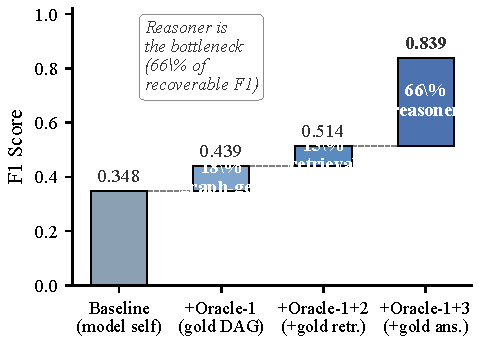
\includegraphics[width=0.98\linewidth]{figures/image6}
\caption{Oracle waterfall on MuSiQue 4-hop (n=200). Substituting gold sub-answers (Oracle-1+3) recovers 66.2\% of the ceiling---the reasoner is the dominant recoverable bottleneck, exactly the failure mode that bidirectional cross-checking targets.}
\label{fig:oracle}
\end{figure}

\begin{table}[t]
\centering
\caption{Oracle waterfall (MuSiQue 4-hop, n=200, Qwen3-8B, full context, paired).}
\label{tab:oracle}
\small
\begin{tabular}{lcccc}
\toprule
Config & EM & F1 & $\Delta$F1 & Share \\
\midrule
Baseline & 0.251 & 0.348 & --- & --- \\
Oracle-1: gold DAG & 0.335 & 0.439 & +0.091 & \textbf{18.4\%} \\
Oracle-1+2: +retrieval & 0.407 & 0.514 & +0.076 & 15.4\% \\
Oracle-1+3: +sub-answers & \textbf{0.780} & \textbf{0.839} & \textbf{+0.325} & \textbf{66.2\%} \\
\bottomrule
\end{tabular}
\end{table}

\noindent\emph{(1) Decomposition itself is significantly valuable.} Oracle-1 (gold decomposition + our reasoner + our aggregation) vs.\ paired CoT-SC on the same 200 samples: Oracle-1 F1 = 0.439 vs.\ CoT-SC F1 = 0.363, \textbf{paired dF1 = +0.075, 95\% CI $[+0.017, +0.134]$, $P(\text{diff}{>}0){=}0.994$}. This is the definitive answer to ``does decomposition matter at all?''---with correct decomposition, the pipeline significantly beats CoT-SC on deep multi-hop.

\noindent\emph{(2) The reasoner is the largest recoverable bottleneck.} Table~\ref{tab:oracle} shows Oracle-1+3 recovers 66.2\% of recoverable F1, dominating graph generation (18.4\%) and retrieval (15.4\%). Since intermediate reasoner errors are the primary loss channel, a verifier that detects inconsistent sub-answers---bidirectional cross-checking---is well matched to the bottleneck.

\noindent\emph{(3) Model-vs-gold decomposition gap, quantified.} Table~\ref{tab:decomp_gap} makes the actionable target explicit. With model self-decomposition, CV2 modestly loses to CoT-SC (dF1 $-0.022$, n.s.); with gold decomposition, the same pipeline significantly beats CoT-SC (dF1 $+0.075$, F1 SIG). The problem is not that decomposition is unhelpful---it is that current 8B-class LLMs leave a $\sim$0.10 F1 gap below the gold ceiling.

\begin{table}[t]
\centering
\caption{Model-generated vs.\ gold decomposition on MuSiQue 4-hop (Qwen3-8B, paired vs.\ CoT-SC). Same benchmark and pipeline; only the decomposition source changes.}
\label{tab:decomp_gap}
\small
\begin{tabular}{lcccc}
\toprule
Decomposition source & $n$ & GERS F1 & $\Delta$F1 & 95\% CI \\
\midrule
Model self-decompose & 85 & 0.348 & $-0.022$ & $[-0.115, +0.071]$ \\
\textbf{Gold (Oracle-1)} & 200 & \textbf{0.439} & \textbf{+0.075} & \textbf{$[+0.017, +0.134]$} \\
\bottomrule
\end{tabular}
\end{table}

\noindent\textbf{Connection to the main results.} On LongBench multi-document QA (\S4.2), multi-passage context lets model-generated decomposition be good enough for the bidirectional cross-check to extract a significant regime advantage. On MuSiQue 4-hop with model self-decomposition, the decomposition-quality gap dominates; the Oracle-1 significance quantifies the achievable ceiling for future depth-planning work.

\subsection{Consistency Score: Structural $\to$ Content}

\begin{figure}[t]
\centering
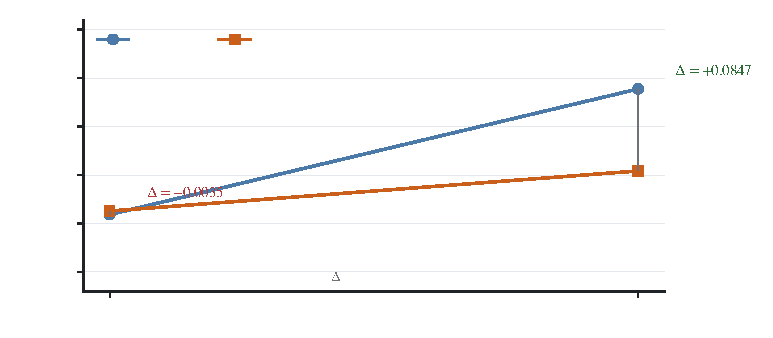
\includegraphics[width=0.95\linewidth]{figures/image2}
\caption{Consistency Score correct/wrong discrimination on HotpotQA n=500. Structural CS clusters around 0.66 for both correct and wrong (discrimination $-0.0035$); adding bidirectional cross-checking separates them (discrimination $+0.0847$, AUROC 0.498$\to$0.589).}
\label{fig:cs}
\end{figure}

Bidirectional cross-checking not only helps end-task performance---it also repairs the Consistency Score itself. Prior graph methods rely on structural graph-validity metrics (connectivity, acyclicity, coverage); on HotpotQA n=500 the structural CS clusters (correct-mean 0.6592, wrong-mean 0.6628, discrimination $-0.0035$, AUROC 0.498)---essentially non-informative because LLM-generated DAGs are almost always legal. After adding the cross-check, discrimination climbs to $+0.0847$ and AUROC to 0.589, upgrading CS from a graph-legality metric to a content self-consistency signal (Figure~\ref{fig:cs}).

\noindent\textbf{Diagnostic, not verifier.} We report honestly that CS remains an imperfect predictor: on GERS-CV2, 156 of 250 CS${=}1.0$ samples are still EM-wrong. High-CS-wrong answers persist because fluent hallucinations agree with themselves. CS is best interpreted as a diagnostic/ranking signal that improves candidate selection, not a standalone verifier; grounded verification remains an open direction (\S\ref{sec:discussion}).

\subsection{Regime Boundary Analysis}
\label{sec:boundary}

We report documented regimes where GERS-CV2 does \emph{not} outperform CoT-SC and analyze why.

\noindent\textbf{Boundary 1: short single-file dense evidence (HotpotQA).} On HotpotQA n=500 under fair full-context evaluation, CoT-SC modestly outperforms GERS-CV2 (F1 0.716 vs.\ 0.683, paired diff $+0.032$ F1 in favor of CoT-SC, 95\% CI $[+0.002, +0.063]$; EM $p{=}0.314$ n.s.). Single-file $\sim$4.7k-character context lets single-pass reading retrieve the bridging entity without decomposition overhead. Per-type breakdown (Table~\ref{tab:hpqa_type}) shows the regime signal even within HotpotQA: on \emph{comparison} questions (structurally similar to LongBench multi-passage), GERS-CV2 outperforms baselines; the aggregate loss comes from \emph{bridge} questions where extraction dominates over reasoning.

\begin{table}[t]
\centering
\caption{HotpotQA per-type EM (n=500). GERS-CV2 wins on comparison-type questions (structurally similar to the LongBench winning regime) but loses on bridge questions where extraction suffices.}
\label{tab:hpqa_type}
\small
\begin{tabular}{lcc}
\toprule
Method & bridge (n=404) & comparison (n=96) \\
\midrule
Zero-Shot & 0.218 & 0.521 \\
CoT-SC & 0.218 & 0.448 \\
\textbf{GERS-CV2} & \textbf{0.240} & \textbf{0.562} \\
\bottomrule
\end{tabular}
\end{table}

\noindent\textbf{Boundary 2: deep bridge-composition (2Wiki bridge\_comp).} On 2WikiMultiHopQA~\citep{ho20202wiki} n=100 diagnostic, GERS-CV2 wins on comparison (F1 0.775 vs.\ Standard CoT 0.815, close) but loses on \emph{bridge\_comparison} (0.524 vs.\ 0.905). The failure mode is reasoner error propagation across a bridge$\to$compare chain (Figure~\ref{fig:type}); an early entity error propagates and inverts the comparison. Bidirectional cross-checking partially mitigates this (0.476$\to$0.524) but does not close the gap---backward pass anchored on a wrong $A$ can still self-agree. This confirms the Oracle-1+3 gap identifying reasoner error propagation as the residual failure mode.

\begin{figure}[t]
\centering
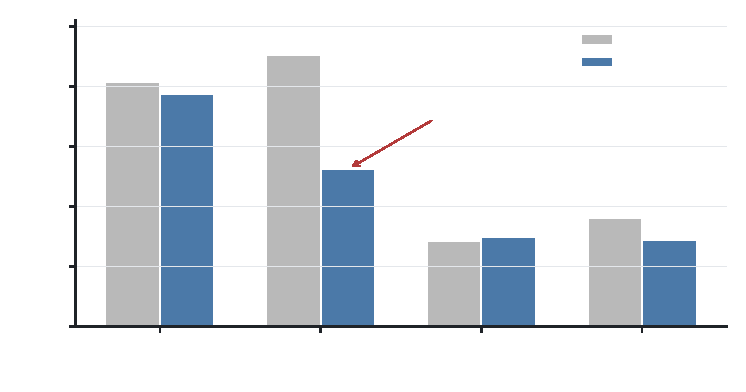
\includegraphics[width=0.98\linewidth]{figures/image5}
\caption{2WikiMultiHopQA per-type F1 (n=100). GERS-CV2 is close on comparison but lags on bridge\_comparison due to reasoner error propagation across the bridge$\to$compare chain.}
\label{fig:type}
\end{figure}

\noindent\textbf{Boundary 3: ultra-long single-narrative (narrativeqa).} Reported in \S4.2: both methods score F1${<}0.24$ with 21--26\% API timeouts at $>$22k tokens---a joint model-capacity ceiling for Qwen3-8B.

\noindent\textbf{Summary.} GERS-CV2 wins where reasoning requires bridging across \emph{multiple passages with heavy distractors} at \emph{5--12k tokens}. It does not help on short single-file QA (HotpotQA bridge), deep composite chains exceeding reasoner error-propagation tolerance (2Wiki bridge\_comp), or contexts beyond model capacity (narrativeqa). This regime coincides with retrieval-augmented multi-document QA.

\subsection{Ablation and Cost}

\begin{table}[t]
\centering
\caption{Component ablation (HotpotQA n=500 paired reference). Each row adds one component to GERS-CV2. Cross-checking is the largest single gain source.}
\label{tab:ablation}
\small
\begin{tabular}{lcc}
\toprule
Config & EM & F1 \\
\midrule
w/o graph execution (CoT-SC + rerank) & 0.264 & 0.372 \\
GERS + adaptive (DAG only) & 0.284 & 0.395 \\
\quad + $K{=}3$ multi-path w/ structural CS & 0.282 & 0.398 \\
\quad \textbf{+ bidirectional cross-check (CV)} & \textbf{0.298} & \textbf{0.409} \\
\quad \quad + confidence weighting (CV2) & 0.302 & 0.413 \\
\bottomrule
\end{tabular}
\end{table}

Table~\ref{tab:ablation} isolates each component in a controlled HotpotQA n=500 paired reference. \emph{Cross-checking is the primary gain source} (DAG-only $\to$ +CV: $+0.014$ EM/$+0.014$ F1, the largest single-component contribution)---exactly the change that also repairs CS discrimination from $-0.0035$ to $+0.0847$. \emph{Structural-CS $K{=}3$ multi-path does not help} (indistinguishable from DAG-only, paired McNemar $p{=}1.000$)---multi-path selection under a non-discriminative score degenerates to random sampling, motivating the cross-check. \emph{Graph execution is the foundation}: removing DAG execution drops to 0.264 EM (below CoT-SC), indicating decomposition must participate in execution, not merely rerank linear traces. \emph{Confidence weighting}: +0.4pt EM ($p{=}1.000$), retained for interpretability.

\noindent\textbf{Cost.} GERS-CV2 uses roughly 2--3$\times$ more LLM calls than CoT-SC ($\sim$6--8 vs.\ 3 per question), corresponding to the $n$ backward-verification calls. Under parallel API, per-question latency is comparable (6.6s vs.\ 8.3s: shorter verification prompts + adaptive routing). We flag this trade-off transparently: for RAG-style multi-document QA the paired-significant regime gains (\S4.2) justify the 2--3$\times$ cost.

\subsection{Case Study}

We illustrate the mechanism with two real cases (Table~\ref{tab:case}). \textbf{Case A (grounded, correct).} ``Were Scott Derrickson and Ed Wood of the same nationality?'' Forward decomposition asks each director's nationality (both ``American''), leading to ``yes''. Reverse verification anchored on ``yes'' + context re-derives both nationalities as ``American''---match. Crossval = 1.0. \textbf{Case B (hallucination detected).} ``Which director had the longest career, Alain Resnais or Scott Sidney?'' Forward pass confidently computes birth/death years (1922, 2014, 1902, 1975) and career lengths---\emph{but these numbers are not in the context}. Reverse verification, re-deriving from context, repeatedly returns ``not in context''---mismatching all 7 forward sub-answers. Crossval collapses to 0.0. Structural CS remains 0.7 (legal DAG) and fails to detect the problem; cross-validated CS reflects the content inconsistency. This is the failure mode that scales up on multi-document long contexts.

\begin{table}[t]
\centering
\caption{Case study: forward/backward sub-answer agreement. Context spans abbreviated.}
\label{tab:case}
\small
\begin{tabular}{lccc}
\toprule
Case & Forward (excerpt) & Backward (excerpt) & New CS \\
\midrule
A: nationality & Amer.\ / Amer. & Amer.\ / Amer. & 1.0 \\
B: career & 1922, 2014, ... & ``not in context'' & 0.0 \\
\bottomrule
\end{tabular}
\end{table}

\subsection{Cross-Model Generalization and Auxiliary Ablations}

\noindent\textbf{Stronger model (Qwen-Plus, n=300).} On Qwen-Plus (HotpotQA n=300), GERS-CV2 EM 0.363, F1 0.496 vs.\ CoT-SC EM 0.367, F1 0.494 (paired diff $-0.004$, $p{=}1.000$). Consistent with the regime hypothesis: as base-model attention improves, CV2's advantage compresses toward zero. GERS-CV2's gain is concentrated on 8B-class models on multi-passage long contexts.

\noindent\textbf{Auxiliary ablations.} (i) Uniform vs.\ downstream-weighted $w_i$: 0.300 vs.\ 0.302 EM, indistinguishable. (ii) 2Wiki at n=300 confirms the bridge\_comparison boundary. (iii) Context-only backward-verification (removing $A$ from anchor): EM 0.300 / F1 0.414---near-identical to answer-anchored (0.302 / 0.413), indicating the end-task gain is not driven by simply feeding $A$ back. (iv) Evidence-grounded variant suppresses inflated CS (0.781$\to$0.730) while preserving EM.

\subsection{Additional Diagnostic Experiments}

For transparency and to document the design-space exploration behind the final GERS-CV2 configuration, we report additional diagnostic experiments.

\noindent\textbf{Symmetric context-budget audit (methodological control).} On HotpotQA with symmetric artificial truncation at 7 budgets (n=200 each, both methods truncated identically), CV2 shows a non-monotone signal (peak dF1 $=+0.060$ at budget 2000, McNemar $p{=}0.054$; n.s.\ at 6 other budgets). This rules out unequal truncation as the explanation for the LongBench gains: the artificial-truncation signal is far weaker than the natural LongBench advantage.

\noindent\textbf{MuSiQue hop-axis with model self-decomposition.} On MuSiQue-original (2/3/4-hop, n=500), model-generated decomposition does not beat CoT-SC at any hop (dF1: 2-hop $-0.008$, 3-hop $-0.062$, 4-hop $-0.022$; all n.s.). Under gold decomposition (Oracle-1) the same benchmark shows significance---the failure is decomposition-quality, not the pipeline, quantifying the $\sim$0.10 F1 model-vs-gold gap (\S4.3, Table~\ref{tab:decomp_gap}).

\noindent\textbf{Rejected variants (design-space audit).} (a) Stepwise NLI verification with re-answer (EASV): +0.004 F1 over Oracle-1 baseline (near-ceiling). (b) Iterative deepening decomposition (IDD): attacks the leaf layer, but depth compression happens at initial decomposition; wrong intervention layer. (c) Per-sub-question BM25 retrieval: F1 0.563 vs.\ full-context 0.683 on HotpotQA (paired dF1 $-0.121$, $p{<}0.001$); top-2 retrieval drops gold paragraphs. (d) Grounded-forward gating (GF-GERS): both lexical and semantic sub-answer check versions underperform plain CV2 on n=20 smoke. These variants informed the final design (full-context, model self-decompose, bidirectional cross-check, confidence-weighted aggregation).

\section{Discussion and Limitations}
\label{sec:discussion}

\noindent\textbf{Content self-consistency, not correctness.} Even after cross-checking, 156 of 250 CS${=}1.0$ HotpotQA samples are EM-wrong and AUROC 0.589 is far from a reliable verifier. CS is a diagnostic/ranking signal, not a standalone verifier; grounded verification (evidence-span extraction, external retrieval agreement, independent NLI) remains open.

\noindent\textbf{Confirmation bias.} Anchoring backward derivation on $A$ risks spurious agreement. We mitigate via (i) explicit ``derive from context'' prompt instruction, (ii) a context-only ablation showing near-identical end-task performance. Adversarial answer perturbation is future work.

\noindent\textbf{Model-scale boundary.} On Qwen-Plus, GERS-CV2 is statistically tied with CoT-SC. As base-model long-context attention improves, single-pass reading closes the gap decomposition currently fills; the regime where the method helps will shift.

\noindent\textbf{Deep-bridge error propagation.} An early sub-answer error propagates and inverts the final answer (visible on 2Wiki bridge\_comp; explained by the Oracle-1+3 gap). Backward pass anchored on a wrong $A$ can still self-agree, limiting cross-checking's coverage of this mode. External-verifier or grounded-forward approaches are natural extensions.

\noindent\textbf{Depth-planning failure and future work.} Our decomposition analysis reveals that 67\% of MuSiQue 4-hop questions are compressed into ${\leq}3$-hop decompositions by current 8B LLMs. This depth-planning failure at the initial decomposition step is a candidate target for future work (depth-prompted decomposition, few-shot 4-hop gold exemplars, decomposition self-consistency over depth).

\noindent\textbf{Sample-size caveat.} LongBench provides $n{=}100$/$n{=}200$ for the target subsets; larger multi-domain long-context benchmarks would tighten confidence intervals. This is the standard LongBench evaluation size and is the natural next step for scaling.

\section{Conclusion}

We propose GERS-CV2, a graph-decomposition method with bidirectional sub-answer cross-checking, and show that it significantly outperforms CoT-SC on the operationally important regime of long multi-document QA (LongBench multifieldqa\_en F1 +0.070 SIG; musique F1 +0.063, McNemar $p{=}0.049$). An Oracle analysis on MuSiQue 4-hop demonstrates that decomposition's value is intrinsic (gold-decomp Oracle-1 vs.\ CoT-SC: +0.075 F1 SIG), with 66\% of recoverable F1 in reasoner error propagation---the exact failure mode bidirectional cross-checking targets. The cross-check upgrades the Consistency Score from a non-discriminative structural metric ($-0.0035$) to a diagnostic content-consistency signal ($+0.0847$, AUROC 0.589). We honestly delineate three regime boundaries (short dense evidence, ultra-long single-narrative, stronger base models), positioning our contribution as a method for the multi-document long-context regime rather than a universal solution. Future work: (i) grounded verification to close the CS$\ne$correctness gap; (ii) depth-aware decomposition to close the model-vs-gold gap quantified in \S4.3; (iii) characterizing the regime shift as long-context LLMs continue to scale.

\bibliography{references}

\end{document}
